\section{DeepSmith}

DeepSmith\footnote{DeepSmith available at: https://chriscummins.cc/deepsmith} is
our open source framework for compiler fuzzing. Figure~\ref{fig:deeptune}
provides a high-level overview. In this work we target OpenCL, though the
approach is language agnostic. This section describes the three key components:
a generative model for random programs, a test harness, and voting heuristics
for differential testing.

\begin{figure}
  \centering
  \includegraphics[width=.75\columnwidth]{img/deepsmith}
  \vspace{-1em}
  \caption{%
  DeepSmith system overview.
  \vspace{-1em}
  }%
  \label{fig:deeptune}
\end{figure}

\subsection{Generative Model}

Generating test cases for compilers is hard because their inputs are highly
structured. Producing text with the right structure requires expert knowledge
and a significant engineering effort, which has to be repeated from scratch for
each new language. Instead, we treat the problem as an unsupervised machine
learning task, employing state-of-the-art deep learning techniques to build
models for how humans write programs. Our approach is inspired by breakthrough
results in modeling challenging and high dimensional datasets through
unsupervised learning~\cite{Raghu2016,Radford2016b,Bowman2015}. Contrary to
existing tools, our approach does not require expert knowledge of the target
language and is only a few hundred lines of code.

\paragraph{Handwritten Programs}

The generative model needs to be trained on a \emph{seed corpus} of example
programs. We automated the assembly of this corpus by mining 10k OpenCL kernels
from open source repositories on GitHub. We used an \emph{oracle compiler} (LLVM
3.9) to statically check the source files, discarding files that are not well-
formed. The main purpose of this step is to remove the need to manually check
that each file selected from GitHub does indeed contain OpenCL. A downside is
that any training candidate which triggers a bug in the LLVM 3.9's front end
will not be included. However, this did not prevent our system from uncovering
errors in that compiler (Section~\ref{subsec:clangs}).

This corpus, exceeding one million lines of code, is used as a representative
sample of OpenCL code from which a generative model can be derived.

\paragraph{Encoder}

The textual representation of program codes must be encoded as numeric sequences
for feeding as input to the machine learning model. Prior machine learning works
have used character-level encodings, token-level encodings, or fixed length
feature vectors. We extend the hybrid character/token-level encoding
of~\cite{Cummins2017b}, in which a programming language's keywords and common
names are treated as individual tokens while the rest of the text is encoded on
a character-level basis. This approach hits a balance between compressing the
input text and keeping the number of tokens in the vocabulary low.

We additionally employed semantic-preserving transformations to simplify the
training programs. First, each source file is preprocessed to expand macros and
remove conditional compilation and comments. Then, all user-declared identifiers
are renamed using an arbitrary, but consistent pattern based on their order of
declaration: $\{a,\allowbreak b,\allowbreak c,\allowbreak \ldots,\allowbreak
aa,\allowbreak ab,\allowbreak ac,\allowbreak \ldots\}$ for variables and
$\{A,\allowbreak B,\allowbreak C,\allowbreak \ldots,\allowbreak AA,\allowbreak
AB,\allowbreak AC,\allowbreak \ldots\}$ for functions. This ensures a consistent
naming convention, without modifying program behavior. Finally, a uniform code
style is enforced to ensure consistent use of braces, parentheses, and white
space. These rewriting simplifications give more opportunities for the model to
learn the structure and deeper aspects of the language and speed up the
learning. On the other hand, some bugs in the preprocessor or front-end might no
longer be discoverable. We reason that this is an acceptable trade-off. For
languages where the corpus can be many orders of magnitude larger, for example,
C or Java, models may be generated without these modifications.

\paragraph{Neural Network}

We use the Long Short-Term Memory (LSTM) architecture of Recurrent Neural
Network to model program code~\cite{Hochreiter1997}. In the LSTM architecture
activations are learned with respect not just to their current inputs but to
previous inputs in a sequence. In our case, this allows modeling the probability
of a token appearing in the text given a history of previously seen tokens.
Unlike previous recurrent networks, LSTMs employ a \emph{forget gate} with a
linear activation function, allowing them to avoid the \emph{vanishing
gradients} problem~\cite{Pacanu2013}. This makes them effective at learning
complex relationships over long sequences~\cite{Lipton2015} which is important
for modeling program code. Our LSTM networks model the vocabulary distribution
over the encoded corpus. After initial experiments using different model
parameters, we found that a two layer LSTM network of 512 nodes per layer
provided a good trade-off between the fidelity of the learned distribution and
the size of the network, which limits the rate of training and inference. The
network is trained using Stochastic Gradient Descent for 50 epochs, with an
initial learning rate of 0.002 and decaying by 5\% every epoch. Training the
model on the OpenCL corpus took 12 hours using a single NVIDIA Tesla P40. We
provided the model with no prior knowledge of the structure or syntax of a
programming language.

\paragraph{Program Generation}

The trained network is sampled to generate new programs. The model is seeded
with the start of a kernel (identified in OpenCL using the keywords
\texttt{kernel void}), and sampled token-by-token. A ``bracket depth'' counter
is incremented or decremented upon production of \texttt{\{} or \texttt{\}}
tokens respectively, so that the end of the kernel can be detected and sampling
halted. The generated sequence of tokens is then decoded back to text and used
for compiler testing.


\subsection{Test Harness\label{sec:test-harness}}

\begin{table*}[t!]
  \footnotesize %
  \centering %
  \caption{%
  OpenCL systems and the number of bug reports submitted to date (22\% of
  which have been fixed, the remainder are pending). For each system, two
  testbeds are created, one with compiler optimizations, the other without.%
  \vspace{-.8em}
  }
  \begin{tabular}{ cllllllR{1cm} | R{1.6cm} }
  \toprule
  \textbf{\#. } & \textbf{Platform} & \textbf{Device} & \textbf{Driver} & \textbf{OpenCL} &
  \textbf{Operating system} & \textbf{Device Type} & \textbf{Open Source?} & \textbf{Bug Reports Submitted} \\
  \midrule
  1 & NVIDIA CUDA & GeForce GTX 1080 & 375.39 & 1.2 & Ubuntu 16.04 64bit & GPU & & 8 \\
  2 & NVIDIA CUDA & GeForce GTX 780 & 361.42 & 1.2 & openSUSE 13.1 64bit & GPU & & 1 \\
  3 & Beignet & Intel HD Haswell GT2 & 1.3 & 1.2 & Ubuntu 16.04 64bit & GPU & Yes & 13 \\
  4 & Intel OpenCL & Intel E5-2620 v4 & 1.2.0.25 & 2.0 & Ubuntu 16.04 64bit & CPU & & 6 \\
  5 & Intel OpenCL & Intel E5-2650 v2 & 1.2.0.44 & 1.2 & CentOS 7.1 64bit & CPU & & 1 \\
  6 & Intel OpenCL & Intel i5-4570 & 1.2.0.25 & 1.2 & Ubuntu 16.04 64bit & CPU & & 5 \\
  7 & Intel OpenCL & Intel Xeon Phi & 1.2 & 1.2 & CentOS 7.1 64bit & Accelerator & & 3 \\
  8 & POCL & POCL (Intel E5-2620) & 0.14 & 1.2 & Ubuntu 16.04 64bit & CPU & Yes & 22 \\
  9 & Codeplay & ComputeAorta (Intel E5-2620) & 1.14 & 1.2 & Ubuntu 16.04 64bit & CPU & & 1 \\
  10 & Oclgrind & Oclgrind Simulator & 16.10 & 1.2 & Ubuntu 16.04 64bit & Emulator & Yes & 7 \\

  \bottomrule
\end{tabular}


  \vspace{-.7em}
  \label{tab:platforms}
\end{table*}

OpenCL is an embedded compute kernel language, requiring host code to compile,
execute, and transfer data between the host and device. For the purpose of
compiler fuzzing, this requires a \emph{test harness} to run the generated
OpenCL programs. At first, we used the test harness of CLSmith. The harness
assumes a kernel with no input and a \texttt{ulong} buffer as its single
argument where the result is written. Only 0.2\% of the GitHub kernels share
this structure. We desired a more flexible harness so as to test a more
expressive range of programs, capable of supporting multi-argument kernels and
generating data to use as inputs.

We developed a harness which first determines the expected arguments from the
function prototype and generates host data for them. At the moment, we support
scalars and arrays of all OpenCL primitive and vector types. For a kernel
execution across $n$ threads, buffers of size $n$ are allocated for pointer
arguments and populated with values {$[1 \ldots n]$}; scalar inputs are given
value $n$, since we observe that most kernels use these for specifying buffer
sizes.

The training programs from which the generative model is created are real
programs, and as such do not share the argument type restrictions. The model,
therefore, may generate correct programs for which our driver cannot create
example inputs. In this case, a ``compile-only'' stub is used, which only
compiles the kernel, without generating input data or executing the compiled
kernel.

Unlike the generative model, this test harness is language-specific and the
design stems from domain knowledge. Still, it is a relatively simple procedure,
consisting of a few hundred lines of Python.

\paragraph*{Test Harness Output Classes}
\begin{figure}
  \centering %
  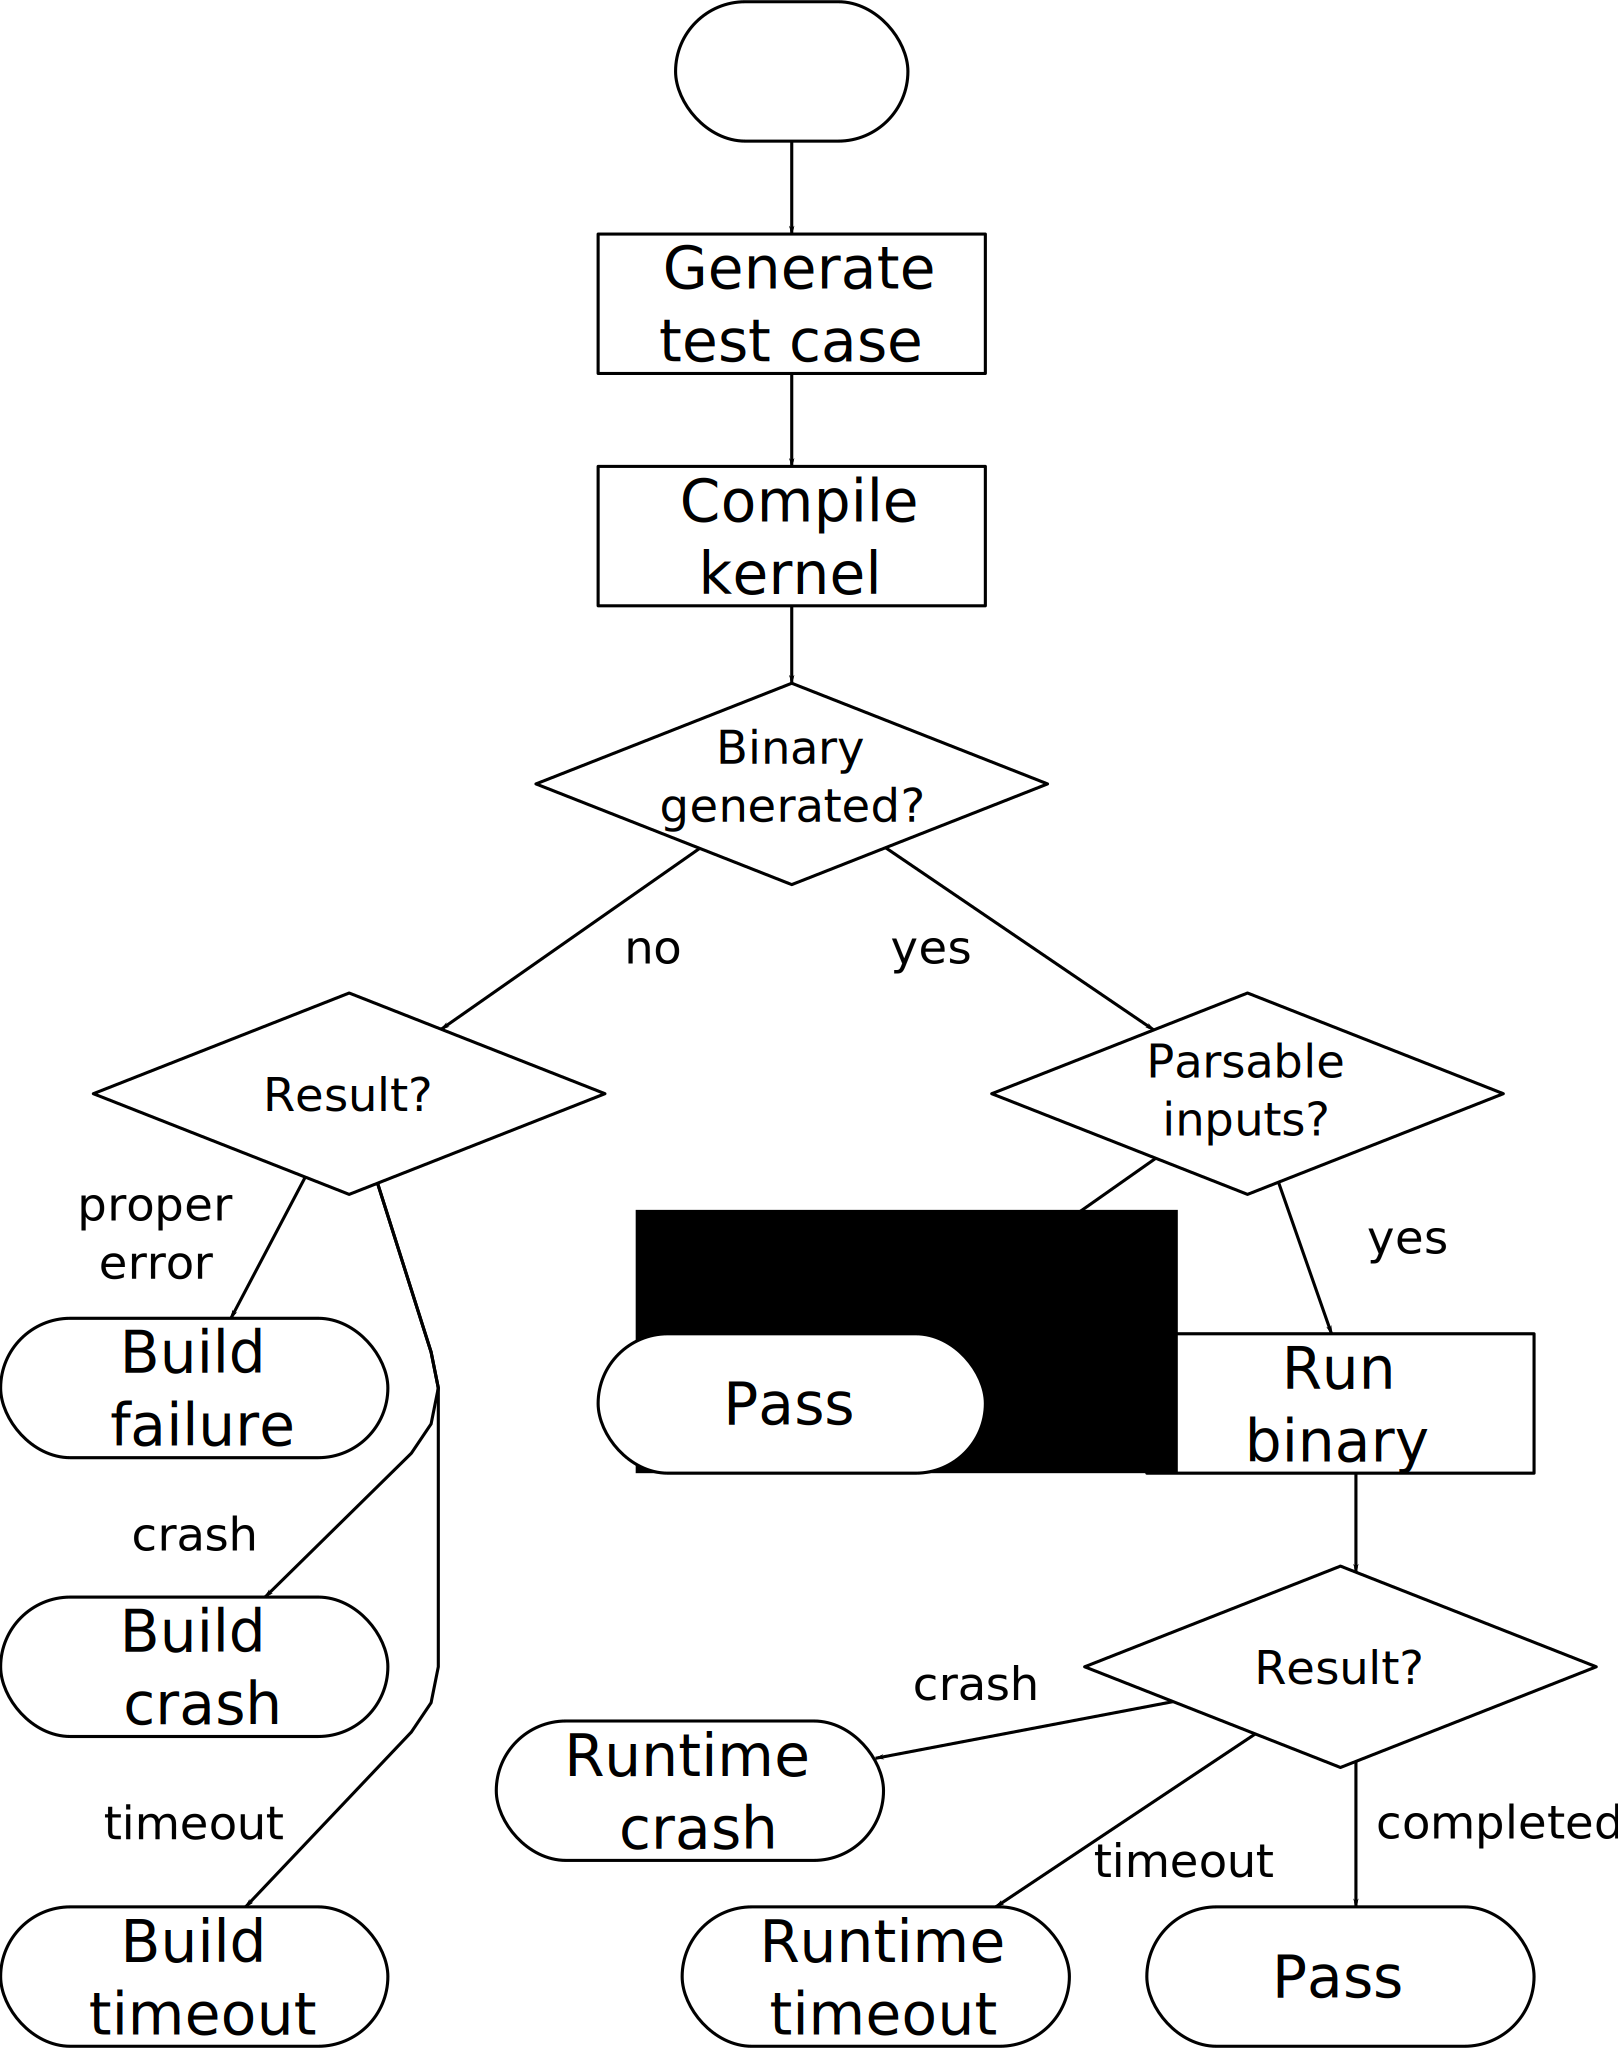
\includegraphics[width=.7\columnwidth]{img/testprocess-long}
  \vspace{-.5em}
  \caption{%
  Test case execution, and possible results.%
  \vspace{-1.5em}
  }%
  \label{fig:test-process}
  %
\end{figure}
Executing a test case on a testbed leads to one of seven possible outcomes,
illustrated in Figure~\ref{fig:test-process}. A \emph{build failure} occurs when
online compilation of the OpenCL kernel fails, usually accompanied by an error
diagnostic. A \emph{build crash} or \emph{build timeout} outcome occurs if the
compiler crashes or fails to produce a binary within 60 seconds, respectively.
For compile-only test cases, a \emph{pass} is achieved if the compiler produces
a binary. For test cases in which the kernel is executed, kernel execution leads
to one of three potential outcomes: \emph{runtime crash} if the program crashes,
\emph{timeout} if the kernel fails to terminate within 60 seconds, or
\emph{pass} if the kernel terminates gracefully and computes an output.

\subsection{Voting Heuristics for Differential Testing}

We employ established Differential Testing methodologies to expose compiler
defects. As in prior work, voting on the output of programs across compilers has
been used to circumvent the \emph{oracle problem} and detect
miscompilations~\cite{McKeeman1998}. However, we extend this approach to
describe not only miscompilations, but also anomalous build failures and
crashes.

When evaluating the outcomes of test cases, build crash (\bc) and build timeout
(\bto) outcomes are of immediate interest, indicative of erroneous compiler
behavior (examples may be found in Section~\ref{subsec:compile-time-defects}).
For all other outcomes, \emph{differential tests} are required to confirm
anomalous behavior. We look for test cases where there is a majority outcome --
i.e. for which some fraction of the testbeds behave the same -- but some testbed
deviates. We use the presence of the majority increasing the likelihood that
there is a `correct' behavior for the test case. In this work, we choose the
majority fraction to be $\ceil{\frac{2}{3}n}$, where $n$ is the number of
testbeds.

An \emph{anomalous build failure} (\abf) or \emph{anomalous runtime crash}
(\arc) occurs if, for a given test case, the majority of testbeds execute
successfully, and a testbed yields a compilation error or runtime crash. An
\emph{anomalous wrong-output} (\awo) occurs if, for a given test case, the
majority of testbeds execute successfully, producing the same output values, and
a testbed yields a result which differs from this majority output. Anomalous
wrong-output results are indicative of \emph{miscompilations}, a particularly
hard to detect class of bug in which the compiler silently emits wrong code.
CSmith is designed specifically to target this class of bug.

\paragraph{False Positives for Anomalous Runtime Behavior}%
\label{subsec:discussions}

Generated programs may contain undefined or non-deterministic behavior which
will incorrectly be labeled as anomalous. CSmith circumvents this problem by
performing complex analyses during generation so as to minimize the chance of
producing programs with undefined behavior. Although similar analyses could be
created as filters for our system, we take a simpler approach, filtering only
the few types of non-deterministic behavior we have actually observed to happen
in practice.

We filter data races, out-of-bounds and uninitialized accesses with
GPUverify~\cite{Betts2012} and Oclgrind~\cite{Price2015}. Some compiler warnings
provide strong indication of non-deterministic behavior (e.g. comparison between
pointer and integer) -- we check for these warnings and filter accordingly.

Floating point operations in OpenCL can be imprecise, so code can produce
different output on different testbeds. For this reason, CSmith and CLSmith do
not support floating point operations. DeepSmith allows floating point
operations but since it cannot apply differential testing on the outputs, it can
detect all results except for the \emph{anomalous wrong-output} results.

The last type of undefined behavior we observed comes from division by zero and
related mathematical functions which require non-zero values. We apply a simple
detection and filtering heuristic -- we change the input values and check to see
if the output remains anomalous. While theoretically insufficient, in practice
we found that no false positives remained.
